\chapter{Materials and Methods}\label{chap:mat_and_methods}
In \autoref{fig:mat_met_overview} a brief overview of the processes applied in this work is displayed. In the coming sections, each compartment will be separately analyzed.

\begin{figure}[H]
	\centering
	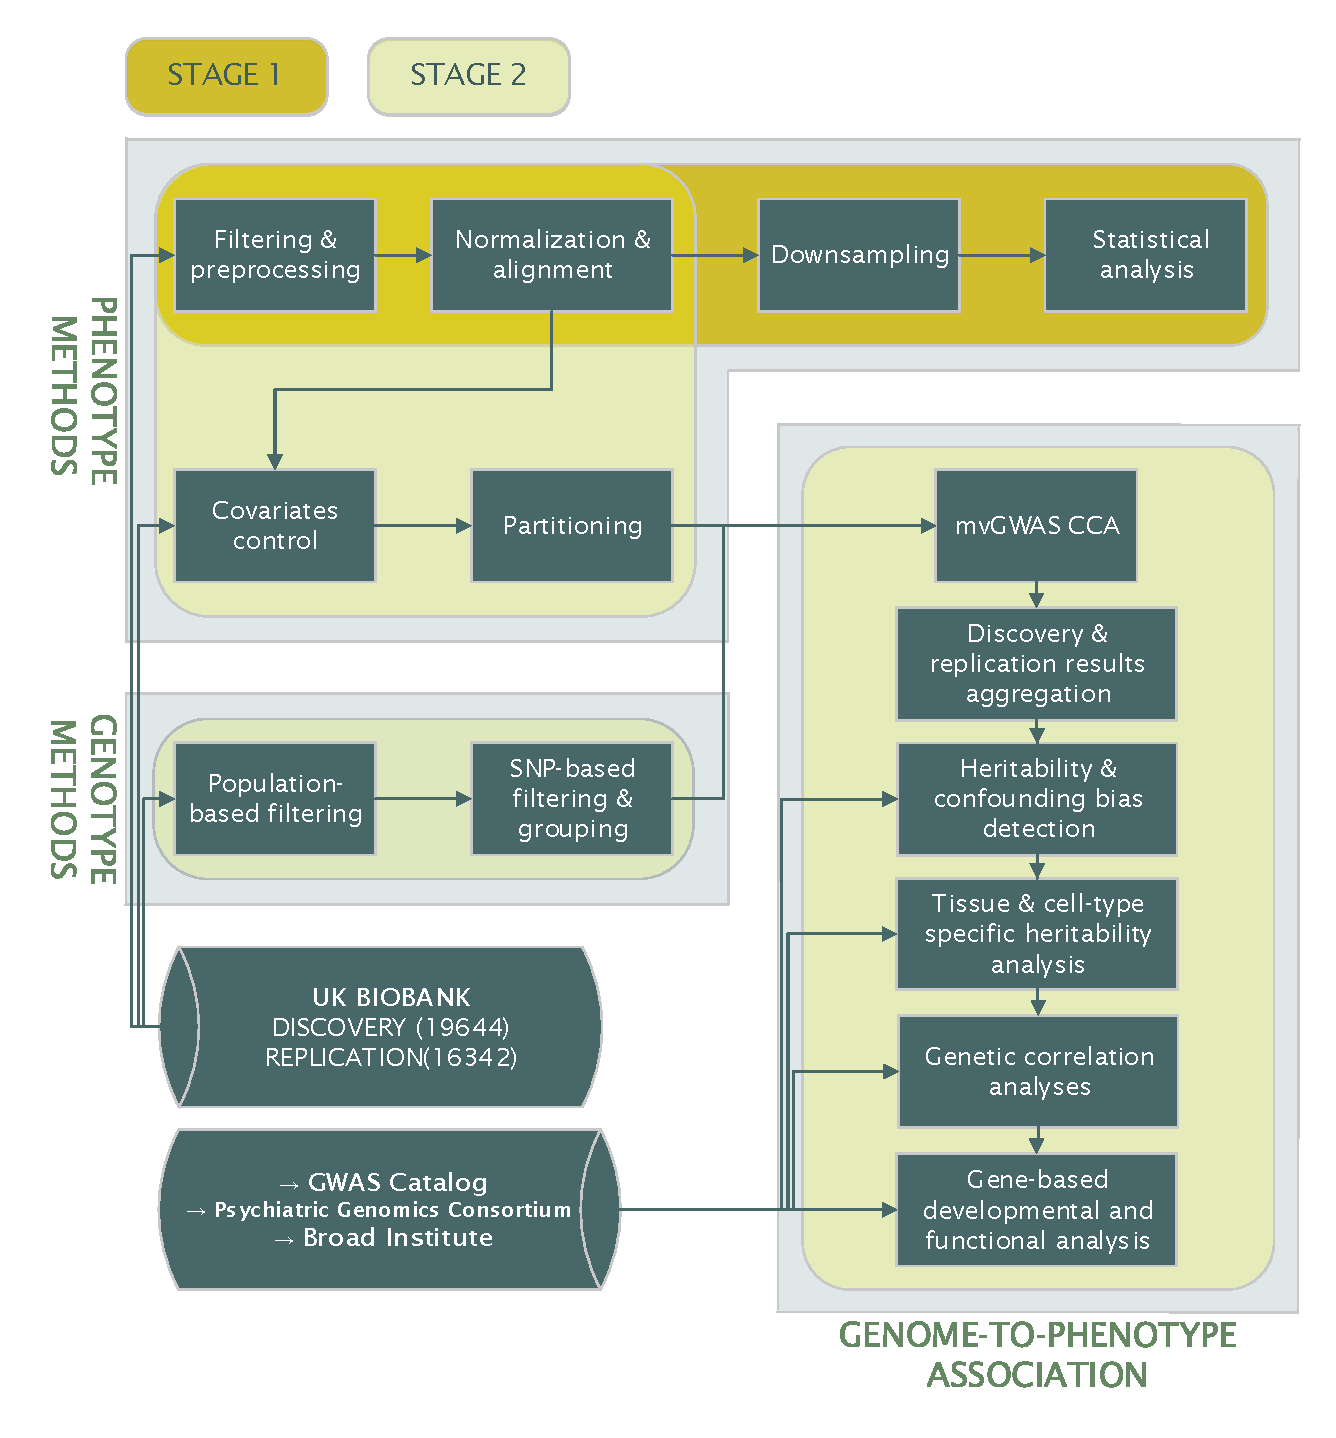
\includegraphics[width=0.8\textwidth]{diagram}
	\caption[Visual overview of methods and materials]{Visual overview of the applied methods and used materials. Stage 1 corresponds to the statistical analysis of brain shape asymmetry. Overlapping stage 2 refers to the steps performed in the genetic and functional studies.}
	\label{fig:mat_met_overview}
\end{figure}


\section{Data description}
\subsection{Primary Data Source}
\label{subsec:primary_data_source}
With the advent of technology capable to collect and process genomes from different individuals in relatively high speed, vast databases targeting human physiology have been constructed. One of the main players in the data collection has been UK Biobank \cite{Bycroft2018}; a large-scale database from a randomized consortium of 500,000 individuals, whose genome has been collected, from whom  48,000 subjects had also participated in brain \ac{mri} collection process, as of December 2020 \cite{Littlejohns2020}. Participants are male and female, with the age range spanning 40 to 69. Apart from \ac{mri} scans and genetic information, of interest are general individual biomarkers that were collected, such as age, height, weight, BMI and blood pressure, as well as information about the imaging process, like date of acquisition, seat height, head (x,y,z) coordinates inside the scanner, and diagnostic center. Those are considered as covariates in the genetic analysis and their effect is assessed and removed. The present study focuses on healthy self-reported white individuals of European ancestry, filtering and preprocessing them based on the work of \citet{Naqvi2021}. Specifically, the discovery dataset, amounting to 19,644 individuals and 9,705,931 \acp{snp}, of the present work is identical to the one used in their study. In addition to that dataset, a smaller one, coming from a different, collected at a later time but under the same protocol, batch of 16,342 individuals is used as a replication dataset during \ac{gwas}.

\subsection{Other sources}
\label{subsec:other_sources}
A 20 samples test-retest \ac{mri} dataset from \ac{hcp} was collected to simulate replications during symmetry analysis. Various other sources are directly used during the meta-analysis, mainly to collect external \ac{gwas} scores. Those were selected from GWAS Catalog \cite{Buniello2019} or the Psychiatric Genomics Consortium and are summarized in the following tables:

\begin{table}[H]
	\centering
	\centerline{
\begin{tabular}{lccc}\toprule
	& \# Cases & \# Controls & Ancestry\\\midrule
\Acs{adhd}\cite{Demontis2019}  & 20,183 & 35,191 & Undefined \\
\Acs{ad}\cite{Jansen2019} & \makecell{24,087 late-onset \\  47,793 with family history} & 383,378 & European \\
\Acs{asd}\cite{Grove2019} & 18,381 & 27,969 & Danish \\
\Acs{bd}\cite{Mullins2021} & 41,917 & 371,459 & European \\
Handedness\cite{DeKovel2019} & 31,856 & 299,181 & British \\
\Acs{mdd}\cite{Guindo-Martinez2021} & 7,264 & 49,373 & European \\
\Acs{ocd} \cite{Arnold2017} & 2,688 & 7,037 & European \\
Red Hair \cite{Morgan2018} & 15,731 & 328,153  & European \\
Schizophrenia \cite{Ripke2014} & 36,989 & 113,075 & European \& Asian \\\bottomrule
\end{tabular}
}
\caption{Qualitative traits \ac{gwas} sources.}
\label{tab:qualit_traits}
\end{table}

\begin{table} [H]
	\centering
	\begin{tabular}{lcc}\toprule
		& \# Individuals & Ancestry\\\midrule
		Cortical surface asymmetry\cite{Sha2021} & 32,256 & European\\
		Cortical surface shape\cite{Naqvi2021} & 19,644 & European \\
		Educational attainment\cite{Okbay2016} &  405,072 & European \\
		Intelligence\cite{Sniekers2017} & 78,308 & European \\
		\acs{lfc}\cite{Mekki2022} & 32,186 & European \\
		Neuroticism\cite{Luciano2018} & 329,821 & European \\
		\bottomrule
	\end{tabular}
	\caption{Quantitative traits \ac{gwas} sources.}
	\label{tab:quantit_traits}
\end{table}
Maybe something surprising presented in \autoref{tab:qualit_traits} is the red hair trait, which was assessed with data from the UK Biobank \cite{Morgan2018}. The reason of its inclusion is that, as the current work's approach is data-driven, significant signal is observed in the gene-based analysis, regarding this trait, raising questions about subpopulation stratification and leading to a deeper investigation of this association. 
As a global reference genome for identifying the \ac{ld} structure and comparing \ac{gwas} from different sources, 1000G (Phase 3) data is used \cite{Auton2015}, with the same reference having been utilized during the phasing (ie. the haplotype inference) and imputation process of UK Biobank genotyping \cite{Bycroft2018}, . For epigenetic studies, the chromatin data from Roadmap Epigenomics \cite{RoadmapEpigenomicsConsortium2015} and ENCODE \cite{Dunham2012} projects are utilized, proposed and preprocessed by \citet{Finucane2018} and offered by Broad Institute, amounting to 489 different tissues. Lastly, the out-of-the-box tools FUMA \cite{Watanabe2017} and STRING\cite{Szklarczyk2021} use their own abundant sets of resources.




\section{Methods applied on Phenotype}
\label{sec:methods_on_pheno}
\subsection{Initial filtering and preprocessing}
\label{subsec:pheno_preproc}
T1-weighted MRI scans are analyzed. The analysis is performed by initially converting the raw DICOM MRI volumetric images to well-defined 3D surface triangular meshes through the pipeline applied by FreeSurfer `recon-all` \cite{Reuter2012} and Ciftify `ciftify-recon-all` commands \cite{Dickie2019}, on a space of 32 thousand vertices, with the average edge length being 2mm. Subsequently, the mid-cortical surface is arbitrarily selected, enabling the distinction of sulci and gyri without over-representing their geometry \cite{Naqvi2021}. After quality control,  the vertices from the sub-cortical part of the surface, referring to corpus callosum connection points, are removed based on a mask derived from the Conte69 atlas \cite{Glasser2011}, getting reduced to 29,759.

\subsection{\Ac{mri} Shapes normalization and alignment}\label{subsec:shape_normalization}
The current work applies principles from general symmetry studies to model cortical asymmetry. For any of these analyses to occur, the aberrations of \ac{3d} shapes produced from \ac{mri} scans need to be considered. \Ac{mri} output is affected by the subject positioning and technical error \cite{Wittens2021}.  Volumetric differences also increase the level of discrepancies among \ac{mri} samples.  To prevent positioning and volume deviations from gravely affecting shape comparisons, a normalization is required\cite{Klingenberg2020}. The samples of the derived 3D triangular mesh are represented as a set of vertices $\mathcal{V}_S$ of predefined dimensionality P, with a single landmark coded in the format of (x,y,z) coordinates. Those are joined together with a predefined faces matrix $\mathcal{E}_S$, with each of its elements containing three indices referring to $\mathcal{V}_S$, with the additional constraint that $S$ is a multiple-connected structure, namely a graph in which there is at least one path joining any two vertices. Shapes normalization is performed through the application of \ac{gpa}. \Ac{gpa} is an algorithm that iteratively performs translation, scaling and rotation on a given set of structures $S$, given initially a reference $S_0$, aiming to minimize the euclidean distance of corresponding points and the average shape. The translation is performed in such a way that the centroid C, defined by $\frac{\sum_{\forall i}{\mathcal{E}_S}_i}{P}$, becomes the system origin. The scaling is such that the centroid size of the normalized $S$ structure, defined by $\sqrt{\sum_{\forall i}{\left|\left|{\mathcal{E}_S}_i-C\right|\right|_2}}$ becomes equal to 1. The transformed samples then belong to what it has been coined as Kendall Space \cite{Klingenberg2020}.  Under the framework of cortical surface analysis, a single hemisphere is considered to be one of the $S$ structures. To apply any symmetry analysis, therefore, one of the individual hemispheres needs to be mirrored on the other side of the midsagittal plane, and then \ac{gpa} is applied to align all hemispheres at once. The mirroring is performed by normalization of right and left hemispheres sets separately, and, then, x coordinate sign inversion of the right hemisphere landmarks. Aligning, finally, the entire dataset marks the end of the shapes normalization for the two tasks, statistical asymmetry analysis and \ac{gwas}, resulting into left ($H_L$) and mirrored right ($H_R$) shapes. In the case of \ac{gwas}, the difference between the left and right landmarks of the aligned shapes $D_A=\mathcal{E}_{H_L}-\mathcal{E}_{H_R}$ is computed, a proxy of \ac{da} defined in \autoref{subsec:stat_methods}, before being reshaped to merge the dimensions of L landmarks and coordinates, resulting an array with size $N\times3L$. This structure plays the role of the asymmetry phenotype in further analysis. 

\subsection{Downsampling}
\label{subsec:downsampling}
An intermediate step is followed when performing cortical symmetry statistical analysis, in order to reduce the computational burden of the process. A rather simple algorithm, in MATLAB context, has been derived, that computes the subset of indices of a given shape S, \textit{approximately} with a given factor, that best describe the downsampled shape $M$ provided from the  proprietary function `reducepatch` output \cite{Lopez2014}. With this method, the analyzed shapes are downsampled by a factor of 10, with the average shape retaining most morphological characteristics. The key idea is to find the one-to-many correspondence between faces from the two meshes. Let $\mathbf{{Cn}_T}$ be the centroids of each face of a shape T. The faces correspondence is found by firstly identifying for each face $x\in \mathcal{E}_M$ a part $S_x$ of S, with $\mathcal{E}_{Sx}\subset \mathcal{E}_S$, joined to the closest, to x, face of S with index $y_{min}(x)=\argmin_{\mathbf{{Cn}_{S}}}\left|\left|\mathbf{{Cn}_{S}}-\mathbf{{Cn}_M}\right|\right|_2$, through a path of utmost 10 edges, that is the desired reduction rate. The faces of $S_x$ are having non-zero entries in the 10th power of the S's adjacency matrix, at the $y_{min}$-th row. Then, the optimal vertex correspondence is found by taking all the vertices corresponding to the faces subset $\mathbf{{V}_{Sx}}$ and identifying which of them is the closest to each of the vertices of x. The resulting downsampled shape R then has the faces of M, but projected on the vertices of S. This mapping allows for instant, although naive and of reduced quality, downsampling of 29,759 to 3,098 landmarks (\autoref{fig:downsampling}).
\begin{figure}[H]
	\centering
	\includesvg[width=\linewidth]{downsampling/reduction}
	\caption[Cortical surface downsampling]{Downsampling indices of original average template using the novel algorithm and specific reduction scales (1/r). As no inter-face edge connectivity criterion is being considered, artifacts occur in the approximated shape, in the form of scars.}
	\label{fig:downsampling}
\end{figure}

\subsection{Symmetry Statistical analysis}
\label{subsec:stat_methods}
Bilateral asymmetry is mainly described using three components in literature \cite{klingenberg2002}\cite{Vingerhoets2021}. \Acf{da}, the main focus of this study, corresponds to the hemispheric side effect, namely how the intrinsic (i.e. genetic) properties of the studied population are manifesting across individuals. Antisymmetry, which is related to the effect where sidedness is random in a population (i.e. left-right pattern is mirrored to a right-left pattern), is not observed in the human cerebral cortex, in contrast to other internal organs positions, or organisms \cite{Neubauer2020}. The third component, \acf{fa}, encompasses any random developmental and environmental effects, that cannot be explained with the existing knowledge. The observed deviations can be statistically linearly modeled as products of two effects, the hemisphere side studied and the individual specimen analyzed, as well as their interaction \cite{klingenberg2002}. Given that the analysis is performed on a pair of symmetric objects, and not on a single symmetric object, this configuration is named \textbf{matching asymmetry analysis}. Formally, based on \cite{VanDongen1999} assuming the presence of replications for each observation per individual, to account for technical error, a mixed linear model representing the aforementioned dependencies is defined as:
\begin{equation}
Y_{ijk} = \mu + \beta + I_i + S_{ij} + E_{ijk}
\end{equation}
where $Y_{ijk}$ is the phenotype of the i-th individual, from the j-th side, under the k-th replication, $\mu$ and $\beta$ are the fixed intercept and fixed side effect respectively, $I_i\sim\mathcal{N}(0,\sigma^2_{ind})$ is the random individual effect,  $S_{ij}\sim\mathcal{N}(0,\sigma^2_{FA})$ is the random side and individual specific effect, matched to \ac{fa}, and $E_{ijk}\sim\mathcal{N}(0,\sigma^2_{ME})$ is the measurement error. Given this definition, a way to measure the statistical significance is performed through an F-test applied on a 2-way nonparametric permutation-based \ac{anova}, to relate the \ac{rss} ratios of effects to observable error terms, and of fluctuating effect to the measurement error. Extra care needs to be given on the determination of the \ac{dof} of each term, given the preprocessing applied to bring the hemispheres surfaces into Kendall shape space \cite{klingenberg2002}.  Specifically, the constructed F-ratios, for each pair of contralateral landmarks coordinates separately, on N individuals and R replications, are:
$$
F_I=\frac{RSS_I}{RSS_S}\text{, }
F_{DA}=(N-1)\frac{RSS_D}{RSS_S}\text{, }
F_{FA}=\frac{2(R-1)N}{N-1} \frac{RSS_S}{RSS_E} 
$$ 
$RSS_I$, $RSS_D$, $RSS_S$ and $RSS_E$ are the rows, columns, interaction and error \acp{rss} respectively, as computed by MATLAB `anova2` function on the $NR\times2$ array that contains in each group of R rows information about each individual. Replications are necessary in such analysis, in order to distinguish the \ac{fa} effect from measurement error, and manage to detect $F_{FA}$. To this end, an \ac{mri} test-retest subset of 20 individuals from HCP is retrieved \cite{VanEssen2013}, and the preprocessing mentioned in \autoref{subsec:pheno_preproc} is performed. For each landmark and coordinate, and for each hemisphere separately, the mean observed replication variance across individuals is computed. Subsequently, assuming that the technical measurement error is normally distributed, an augmented dataset is produced for the \ac{mri} samples in the UK Biobank dataset. Three $(R=3)$ replications per individual are generated by sampling from the identified distributions.

While simple \ac{anova} bases the F-score significance on the assumption of normality, permutation-based \ac{anova} makes no assumptions on the underlying distribution \cite{Anderson2001}. Instead it bases significance of a F-statistic on the number of permutations which resulted in F-scores equal or higher than the F-statistic measured in the simple \ac{anova} scenario on the original data, divided by the total number of permutations \cite{Klingenberg1998}. By definition, the observable p-value resolution is the reciprocal of the permutations number. This is introduced in the fraction described above by adding 1 to the nominator and denominator, namely considering the non-permuted case as well. Let N be the number of individuals. A reshaping operation is performed, after which the set of size L landmarks becomes a set of size 3L coordinates per individual per side, in other words a \ac{3d} dataset. The permutations are generated considering each time the dimension being investigated, pursuing biologically feasible result when possible; for assessing the individual effect and computing $RSS_I$, the hemispheres are randomly shuffled across individuals  ($N^{3RL}$ possible orderings); for the side effect test and $RSS_{D}$ measurement, landmarks of each individual are reassigned a random side ($2^{NRL}$ configurations); for the fluctuating effect, quantified by $RSS_{FA}$, the whole dataset is randomly permuted ($(6NRL)!$ orderings). As it can be foreseen, a handicap of the method is the largely unequal size of the possible permutations among the components analyses. This fact renders the last test more sensitive to assign low p-values to each landmark, as the configuration that could possibly produce a better f-score is exponentially less likely to be selected. However, it is worth noting that in all tests the possible cases number is prohibitively large, and that analyses in Monte Carlo simulations, suggest the size of 1000 replications as good enough \cite{Marozzi2004}. 

The consecutive analysis has also been demonstrated in the work of \citet{Vanbiervliet2022}. 1000 replications are selected to test the significance of each asymmetry component, which means that the analysis is computationally intensive, but facilitated by the downsampling described in \autoref{subsec:downsampling}. Five random subsets of 50 samples are collected from the discovery dataset. The number of samples is chosen experimentally, as it was observed that the size of 1000 replications is actually not enough for larger datasets and the method is generally sensitive in assigning high significance (p-value<0.05) to each landmark, the larger the set size assessed. A number of different random subsets is selected, so that to reduce the effect of cherry-picking. The final counts are computed to be the average of the experimental iterations.


\subsection{Covariates control}
In the case of \ac{gwas}, variance caused because of non-genetic factors needs to be excised from the underlying data. To this end, covariates adjustment is performed, by retrieving the residue of a \ac{plsr} \cite{Guebel2013} describing $D_A$ relatively to the factors mentioned in \autoref{subsec:primary_data_source}, along with the 20 genetic \acp{pc}, to account for population stratification and reduce confounding biases (\autoref{tab:covariates}).
\begin{table} [H]
	\centering
	\begin{tabularx}{\textwidth}{ |Y|Y| }
		\hline
		age(1) & age squared(1)\\
		\hline
		height(1) & weight (pre-imaging)(1)\\
		\hline
		diastolic blood pressure(1) & systolic blood pressure(1)\\
		\hline
		date of measurement(1) & genetic \acp{pc} (20))\\
		\hline
		\multicolumn{2}{|c|}{volumetric scaling from T1 head image to standard space(1)}\\
		\hline
		\multicolumn{2}{|c|}{X-position of center-of-gravity of brain mask in scanner coordinates(1)}\\
		\hline
		\multicolumn{2}{|c|}{Y-position of back of brain mask in scanner coordinates(1)}\\
		\hline
		\multicolumn{2}{|c|}{Z-position of center-of-gravity of brain mask in scanner coordinates(1)}\\
		\hline
		\multicolumn{2}{|c|}{Z-position of table/coil in scanner coordinates(1)}\\
		\hline
		\multicolumn{2}{|c|}{one-hot encoded assessment location (21)} \\
		\hline
		\multicolumn{2}{|c|}{left \& right hemisphere centroid sizes prior scaling (2)}\\
		\hline
	\end{tabularx}
	\caption[Covariates used to control phenotype]{Covariates used to control phenotype, totaling 57. Numbers in parenthesis show the dimensionality of each covariate.}
	\label{tab:covariates}
\end{table}



\subsection{Shapes Partitioning}
The present work evaluates the brain asymmetry genetic landscape in a coarse-to-fine segmentation, through \acf{hsc}. The technique has been used in a number of different related phenotypic studies \cite{Claes2018}\cite{Naqvi2021}, yielding results that are in accordance with the underlying anatomic features. The main reason behind this partitioning is the intrinsic complexity of the studied phenotype, eliciting expected differences in the genomic profiles of each cerebral cortex region. This type of distance-based clustering is governed by the least quantity of assumptions, regarding the shape or form of the cluster \cite{VonLuxburg2007}. The partitions' genetic juxtaposition is valuable for identifying which regions share similar significant genetic loci, highlighting the corresponding genes contribution, or showcasing the specialization of certain regions that share little to no similarities with their neighbors.

\Ac{hsc} is an unsupervised method of iterative partitioning, that makes use of the distance matrix eigenvectors \cite{Ng2002}. The distance matrix between pairs of rows of $D_A$, across individuals, is constructed using RV coefficients \cite{Robert1976}, a generalization of Pearson correlation in N-dimensional space. The resulting matrix gets enhanced pairwise similarities, by becoming sharper through the application of the Laplacian transformation dictated by the Shi-Malik method \cite{Shi2000}. The eigenvectors of the matrix are computed and Kmeans++ clustering \cite{Arthur2007} is applied with 2 clusters. The process is repeated on each cluster for a desirable amount of levels, resulting into a binary tree structure (i.e. each parent shape is partitioned into two children). In the current study, a level-4 partitioning is performed, resulting into a tree of 31 partitions, with the root partition, the entire hemisphere, included. Subsequently, the rows of $D_A$ corresponding to each of those partitions are transformed by \ac{pca}, keeping maximally 500 \acp{pc} that explain at most 80\% of the variance, resulting into a structure $P_A$ that contains 31 arrays, ${P_A}_i,i=1..31$, one for each partition, with varying dimensionality. The last step is not only performed for reasons of dimensionality reduction and computational efficiency, but also to ensure that the resulting phenotypic traits are orthogonal with each other, and therefore compatible for \ac{ldsc} analyses, discussed in \autoref{subsec:ldsr}. The partitioning is derived by the discovery dataset only, so that the \ac{gwas} results between discovery and replication datasets correspond to the same partitions and are directly comparable. The computed clustering is subsequently compared to the \ac{dk} atlas parcellation, through a symmetric measure of similarity called \ac{nmi}. Let $U:=\{\mathbf{v_i}\},i=1..n_{DK}$ and $V:=\{\mathbf{{v_j}}\},j=1..31$ be the supersets of sets of indices in $\mathcal{V}_S$ associated to partitions by \ac{dk} atlas and  \ac{hsc} respectively. Then, the \ac{nmi} score is:
$$
\NMI(U,V):=\frac{1}{S}\sum_{i=1}^{|U|} \sum_{j=1}^{|V|} \frac{|U_i\cap V_j|}{N}
\log\frac{N|U_i \cap V_j|}{|U_i||V_j|}
$$
where in this study the normalizing factor S, generally variable \cite{Strehl2003}, is defined as the square root of the product of the sets entropies, namely  
$$
S:=\sqrt{\sum_{i=1}^{|U|}\left(|U_i|log|U_i|\right)\sum_{j=1}^{|V|}\left(|V_j|log|V_j|\right)}
$$
This score is by definition independent on the ordering and the number of the labels. However, a differential number of labels which is expected between the measured labels affects the maximally possible result. Therefore, the score is further normalized by scaling it by the approximate (based on integer division) theoretical maximum score that can observed, if each lesser partitioning does not `share`, in correspondence, any labels of the greater partitioning, apart from a single placeholder label, to account for integer division.
\section{Methods applied on genotype}
\subsection{Population-based filtering}
\ac{pca}, using as reference data the 1000G (Phase 3), is applied to select European individuals only. First, \acp{snp} in \ac{ld}, as computed by PLINK 1.9 with parameters 50 variant window-size, 5 variant step size and 0.2 $r^2$, are excluded from the reference dataset. KMeans algorithm is fitted on 25 \acp{pc} of the reference dataset. Then, only individuals from discovery and replication datasets that are included in the clusters with a EURO label are considered. The individuals identifiers of the genotype are consecutively matched to those in the phenotype.

\subsection{\acs{snp}-based filtering and grouping}
\label{sub:snpbased_filt}
 In addition, \acp{snp} referring to indels, with low genotyping rate (<50\%) , low \ac{maf} $<1\%$ (i.e. corresponding to rare alleles), or not in Hardy-Weinberg equilibrium (P<10.6) are excluded from the analysis. Subsequently, the \ac{ld} filtering applied on the reference dataset is also done for the remaining \acp{snp} of the discovery and replication data. The filtered discovery and replication datasets contain 9,705,931 and 8,305,363 variants respectively. The multi-allelic \acp{snp} rows are grouped together, so that single association test is applied.

\section{Genome-to-phenotype association}
\subsection{\acs{mvgwas} \acs{cca}}
For each i-th partition, \ac{cca} is applied between each \ac{snp} and ${P_A}_i$. To accelerate the \ac{gwas} process, missing values on snp-level were substituted with the mean observed value. The reason behind the acceleration resides in the way \ac{cca} finds the vectors $\vec{a}$,$\vec{b}$  that maximize $corr(a^TX,b^TY)$, or, alternatively, the linear combinations of the input random variables that have maximum correlation. A step of this process is the calculation of the \ac{svd} of both X and Y matrices. If X and Y are the phenotype and genotype respectively, the matrix corresponding to X remains the same throughout the \ac{gwas}, if no missing values exist in the dataset, so the \ac{svd} is required to be computed only once. On the other hand, if missing values are considered in Y, the \ac{svd} of a subset of X needs to be computed for every different \ac{snp} `missingness pattern`, which was identified to be of the order of magnitude of the sample size for the discovery dataset, given the large sample size. The mean substitution greatly affects the computational resources and time required to perform the analysis, reducing them by at least twenty-fold, without an observable effect on the quality of the results, as discussed in \autoref{chap:results}.
The \ac{cca} operation is repeated for both discovery and replication datasets. The produced $\chi^2$ scores are transformed into the quantity dictated by multivariate \ac{ldsc} analysis. The resulting p values are transformed into -log10P values and the \ac{gwas} results are compared qualitatively, as well using \ac{ldsc} genetic correlation analysis.

\subsection{Discovery and replication results aggregation}
Once the comparisons between the results from discovery and replication datasets are made, they are aggregated into a single output, with the p-values combined using Stouffer's method. This method is applied by first projecting the p-values corresponding to the i-th sample into z-scores, through the calculation of the complementary inverse error function $\erfc^{-1}$ of $p_i=\{{p_i}_1,{p_i}_2\}$. The combined p-value ${p_c}_i$ then is:
$$
 {p_c}_i= \erfc\left(\frac{\sum\limits_{k=1}^2 \erfc^{-1}({p_i}_k)}{\sqrt{2}}\right)
$$
Apart from this, the $\chi^2$ scores are summed, under the theoretical basis that the sum of two independent $\chi^2$ values with $d_1$ and $d_2$ \acp{dof} respectively follows a $\chi^2$ distribution with $d_1+d_2$ \acp{dof}.

\subsection{Heritability and confounding bias detection}
\label{subsec:ldsr}
The \ac{ld} between two alleles $A$ and $B$ from different loci is generally quantified using one of the following values: 
\begin{itemize}
	\item{
		the coefficient of linkage disequilibrium $\mathcal{D}$:
		$$
		\mathcal{D} := p_{AB} - p_Ap_B
		$$
		with $p_{AB}$ referring to the haplotype AB frequency and $p_i$ to the frequency of allele i. This coefficient is scaled by theoretical maximum $\mathcal{D}$, $\mathcal{D}_{max}$, to render it independent of the per-pair frequencies magnitudes, producing $\mathcal{D}'$.
	}
	\item{
		the genetic correlation $r^2$, a proxy of the Pearson coefficient, defined by:
		$$
		r^2:= \frac{\mathcal{D}}{p_A(1-p_A)p_B(1-p_B)}
		$$
	}
\end{itemize}
Based on simulations, it has been shown that $\mathcal{D}'$ is inflated when the sample size is small or the minor allele is rare \cite{Teare2002}, thus genetic correlation is generally preferred.  In a seminal research work from \citet{Bulik-Sullivan2015}, it was found that there is a closed mathematical expression that connects the j-th allele $\chi^2$ expected value  with the average heritability explained per \ac{snp} $h$ and its \ac{ld} score, defined by $\sum_k{{r^2_{jk}}}$, $r^2_{jk}$ being the $r^2$ of the j-th with the k-th allele:
$$
E[\chi^2|l_j] = \frac{Nh^2l_j}{M} + N\alpha + 1
$$
$\alpha$ is the contribution of population-related effects, such as population stratification, that are not being controlled, known as confounding biases. The gains from this regression are dual; a measurement of heritability can be obtained by estimating the slope, and the confounding bias effect can be measured by the intercept. This formula, which originally referred to a univariate phenotype, was extended in \cite{Naqvi2021} to incorporate D-dimensional multivariate traits:
$$
E\left[\frac{\chi^2_j}{D\left(1+\frac{\chi^2_j}{N}\right)}\right] = \frac{N-1}{P}\left(\frac{\sum_{d=1}^{D}h_d^2}{D}\right)l_j +1 + O\left(\frac{1}{N}\right)
$$
where $O(1/N)$ term is corresponding to the confounding biases effect. Therefore, this tool is used to estimate heritability and confounding biases, per partition, from the combined \ac{gwas} results.
The basic underlying assumptions, or limitations, of such a model are:
\begin{itemize}
	\item{The \ac{snp} heritability follows a uniform distribution, i.e. it is on average the same genome-wide. Extensions have been made to relax this, generally wrong \cite{Trynka2013}, assumption, by considering partitions of \acp{snp} separately and doing what is known as stratified \ac{ldsr} \cite{Finucane2015,Finucane2018}.}
	\item{Each \ac{snp} effect is assessed independently from the rest, therefore no between-\acp{snp} interactions can be included in the computation.}
	\item{The covariance matrix of the phenotype equals the identity matrix multiplied by N, that is the studied traits are orthogonal to each other.}
\end{itemize}
Another limitation of \ac{ldsr} is that the heritability is under-estimated when the effective sample size is small\cite{Lee2018}.


\subsection{Tissue and cell-type specific heritability analysis}
As mentioned in \autoref{subsec:ldsr}, extensions have been devised to account for different heritability profiles of disparate biological and functional regions. \citet{Finucane2018} incorporate the notion of chromatin regulation and gene expression profiles in \ac{ldsc-seg}. Let m be the number different gene expression profiles, each on a separate tissue or a cell type, an annotation class. For each of those a set of genes, corresponding to a set of \acp{snp} $K_j,(j=1..m)$, has been found to be significantly enriched, relatively to the rest of the comparison group. The discussed extension is of the form:
$$
E\left[\chi^2_i\right]= N \sum_j{\tau_j l(i,j)} + N \alpha + 1
$$
with the \ac{ld} score of the i-th \ac{snp} for the j-th genes cluster $l(i,j)$ being defined as $\sum_{k \in K_j} r^2_{ik}$. $\tau_j$ is the estimated coefficient per annotation class and explains the signed effect of each class on the heritability of the observed phenotype. In other words, the coefficient $\tau_j$ relates the cumulative \ac{ld} effect of the j-th set of \acp{snp} with the observed capacity of the i-th \ac{snp} to affect the phenotypic trait. 

Under this framework, in the present study, a significant association is sought between chromatin regulation studies related to gene expression, to identify the degree under which the identified significant \acp{snp} effects are also likely to be regulated by epigenetic modifications, using the same dataset used by \citet{Finucane2018}, as mentioned in \autoref{subsec:other_sources}.

\subsection{Genetic correlation analyses}
\label{subsec:gencorr}
\citet{Bulik-Sullivan2015_cor} also invented a way to utilize \ac{gwas} scores produced for two different traits as a proxy to relate the genetic correlation of these traits, namely the extent over which the two characteristics are being regulated by similar genetic drivers:
$$
E[z_{1j}z_{2j}|l_j] = \frac{\sqrt{N_1N_2}\rho_g}{M}l_j + \frac{\rho N_s}{\sqrt{N_1N_2}}
$$
The conversion between $\chi^2$ with 1 \ac{dof} and $z$ score values is straightforward, as, by definition, the square of a standard normal distribution follows the $\chi^2$ one with 1 \ac{dof}. In other words, the equation above retrogresses to the \ac{ldsr} one, if traits 1 and 2 are considered the same. With \ac{ldsc}, seemingly independent phenotypes can be compared, testing for pleiotropic \ac{snp} effects and discovering novel biological pathways \cite{Bulik-Sullivan2015_cor}. However, a main limitation of the \ac{cca} \ac{mvgwas} analysis does not contain information about the direction of the effect of a variant on a trait, and such an event is not considered during the derivation of the aforementioned equation \cite{Bulik-Sullivan2015}. Instead, Spearman correlation can be used, to relax the check by testing for monotonic, and not linear, relationships. To this end, LD blocks from the work of \citet{Berisa2016}, retrieved from haplotypic information occurring in the 1000G (Phase 3),  are used to perform an average aggregation of the p-values observed per trait and subsequent monotonicity assessment based on Spearman correlations. A P-value for the correlation process is also produced by comparing bootstrapping spearman correlation variance with the observed correlation.

The aforementioned method, also applied by \citet{Naqvi2021}, is used to relate the \ac{gwas} scores presented in \autoref{subsec:other_sources}. One of those comparisons is done versus the work from \citet{Sha2021}, with the aim to quantitatively relate the results presented there to the current study. In addition, as an internal measure of similarity, it is applied to measure the degree of concordance between the results presented by the discovery and the replication dataset.  

\subsection{Gene-based developmental and functional analysis}
\label{subsec:func_mat_methods}
Last but crucial step, analyses at the gene level are performed. The focus is mainly shifted on 5 partitions; the entire hemisphere, and the 4 ones on the second level, as greater discrepancies in \ac{gwas} are identified among partitions at that level relatively to others. The subsequent analysis refers to the process applied on each partition separately.

Initially, underlying gene sets are retrieved, in the exact same way as it was done by \citet{Sha2021}. More specifically, FUMA toolbox SNP2GENE  utility is used \cite{Watanabe2017}, by accumulating the outputs of positional, eQTL and chromatin interaction mapping, with default parameters only taking into consideration brain-related samples when dimmed necessary \cite{Sha2021,Watanabe2017}. 

Lead \acp{snp} are also retrieved by applying a \ac{grm} $r^2$ upper cutoff of 0.1 on the list of significant \acp{snp}, selected imposing a $5\times 10 ^ {-8}$ threshold on the produced p-values $\mathbf{p_c}$. A further extension of the gene sets is achieved by using GREAT tool \cite{McLean2010}, supplying it with the identified lead \acp{snp}. This tool models possible gene regulatory domains based on empirical evidence and assigns \acp{snp} in such intronic regions to the corresponding genes \cite{McLean2010}.

Leveraging the power of another statistical tool through FUMA, MAGMA, a time-dependent analysis is performed, identifying the degrees under which identified genes are enriched in genetic expression profiles from brain tissues from different developmental stages \cite{DeLeeuw2015}. MAGMA gene-set analysis uses the full distribution of \ac{snp} p-values, hence it is fundamentally different from a \ac{gsea} kind of test. However, long-range relationships, assessed and introduced by the methodologies of FUMA and GREAT, defined above, are not considered. Instead, MAGMA process examines the joint association signals of all \acp{snp} within a given gene, in a 100kb region, while considering the \ac{ld} between those \acp{snp} \cite{DeLeeuw2015,Sha2021}.

The resulting gene set is supplied to the FUMA GENE2FUNC process, where a variety of \acp{gsea} takes place \cite{Watanabe2017}, extracting functional relationships with \ac{go} terms, biological pathways, GWASCatalog traits and differentially expressed tissue-specific gene sets. Concurrently, the identified gene set protein interactions are graphically represented and significantly enriched publications are identified using STRING suite \cite{Szklarczyk2021}. Reactome GO enrichment through PANTHER statistical overrepresentation test \cite{Mi2019}, with Fisher's exact test without correction, is used to annotate large clusters identified in STRING proteins network, produced using MCL algorithm with inflation 2.

	


